\section{Motivación y Objetivos}

\begin{frame}
  \begin{center}
	\Huge ¿QUE ES UNA TRANSMISIÓN \textit{OFDM}?
  \end{center}
\end{frame}

\begin{frame}
  \uncover<1-4>{
    \begin{center}
	  \advance\leftskip-0.2cm
	  {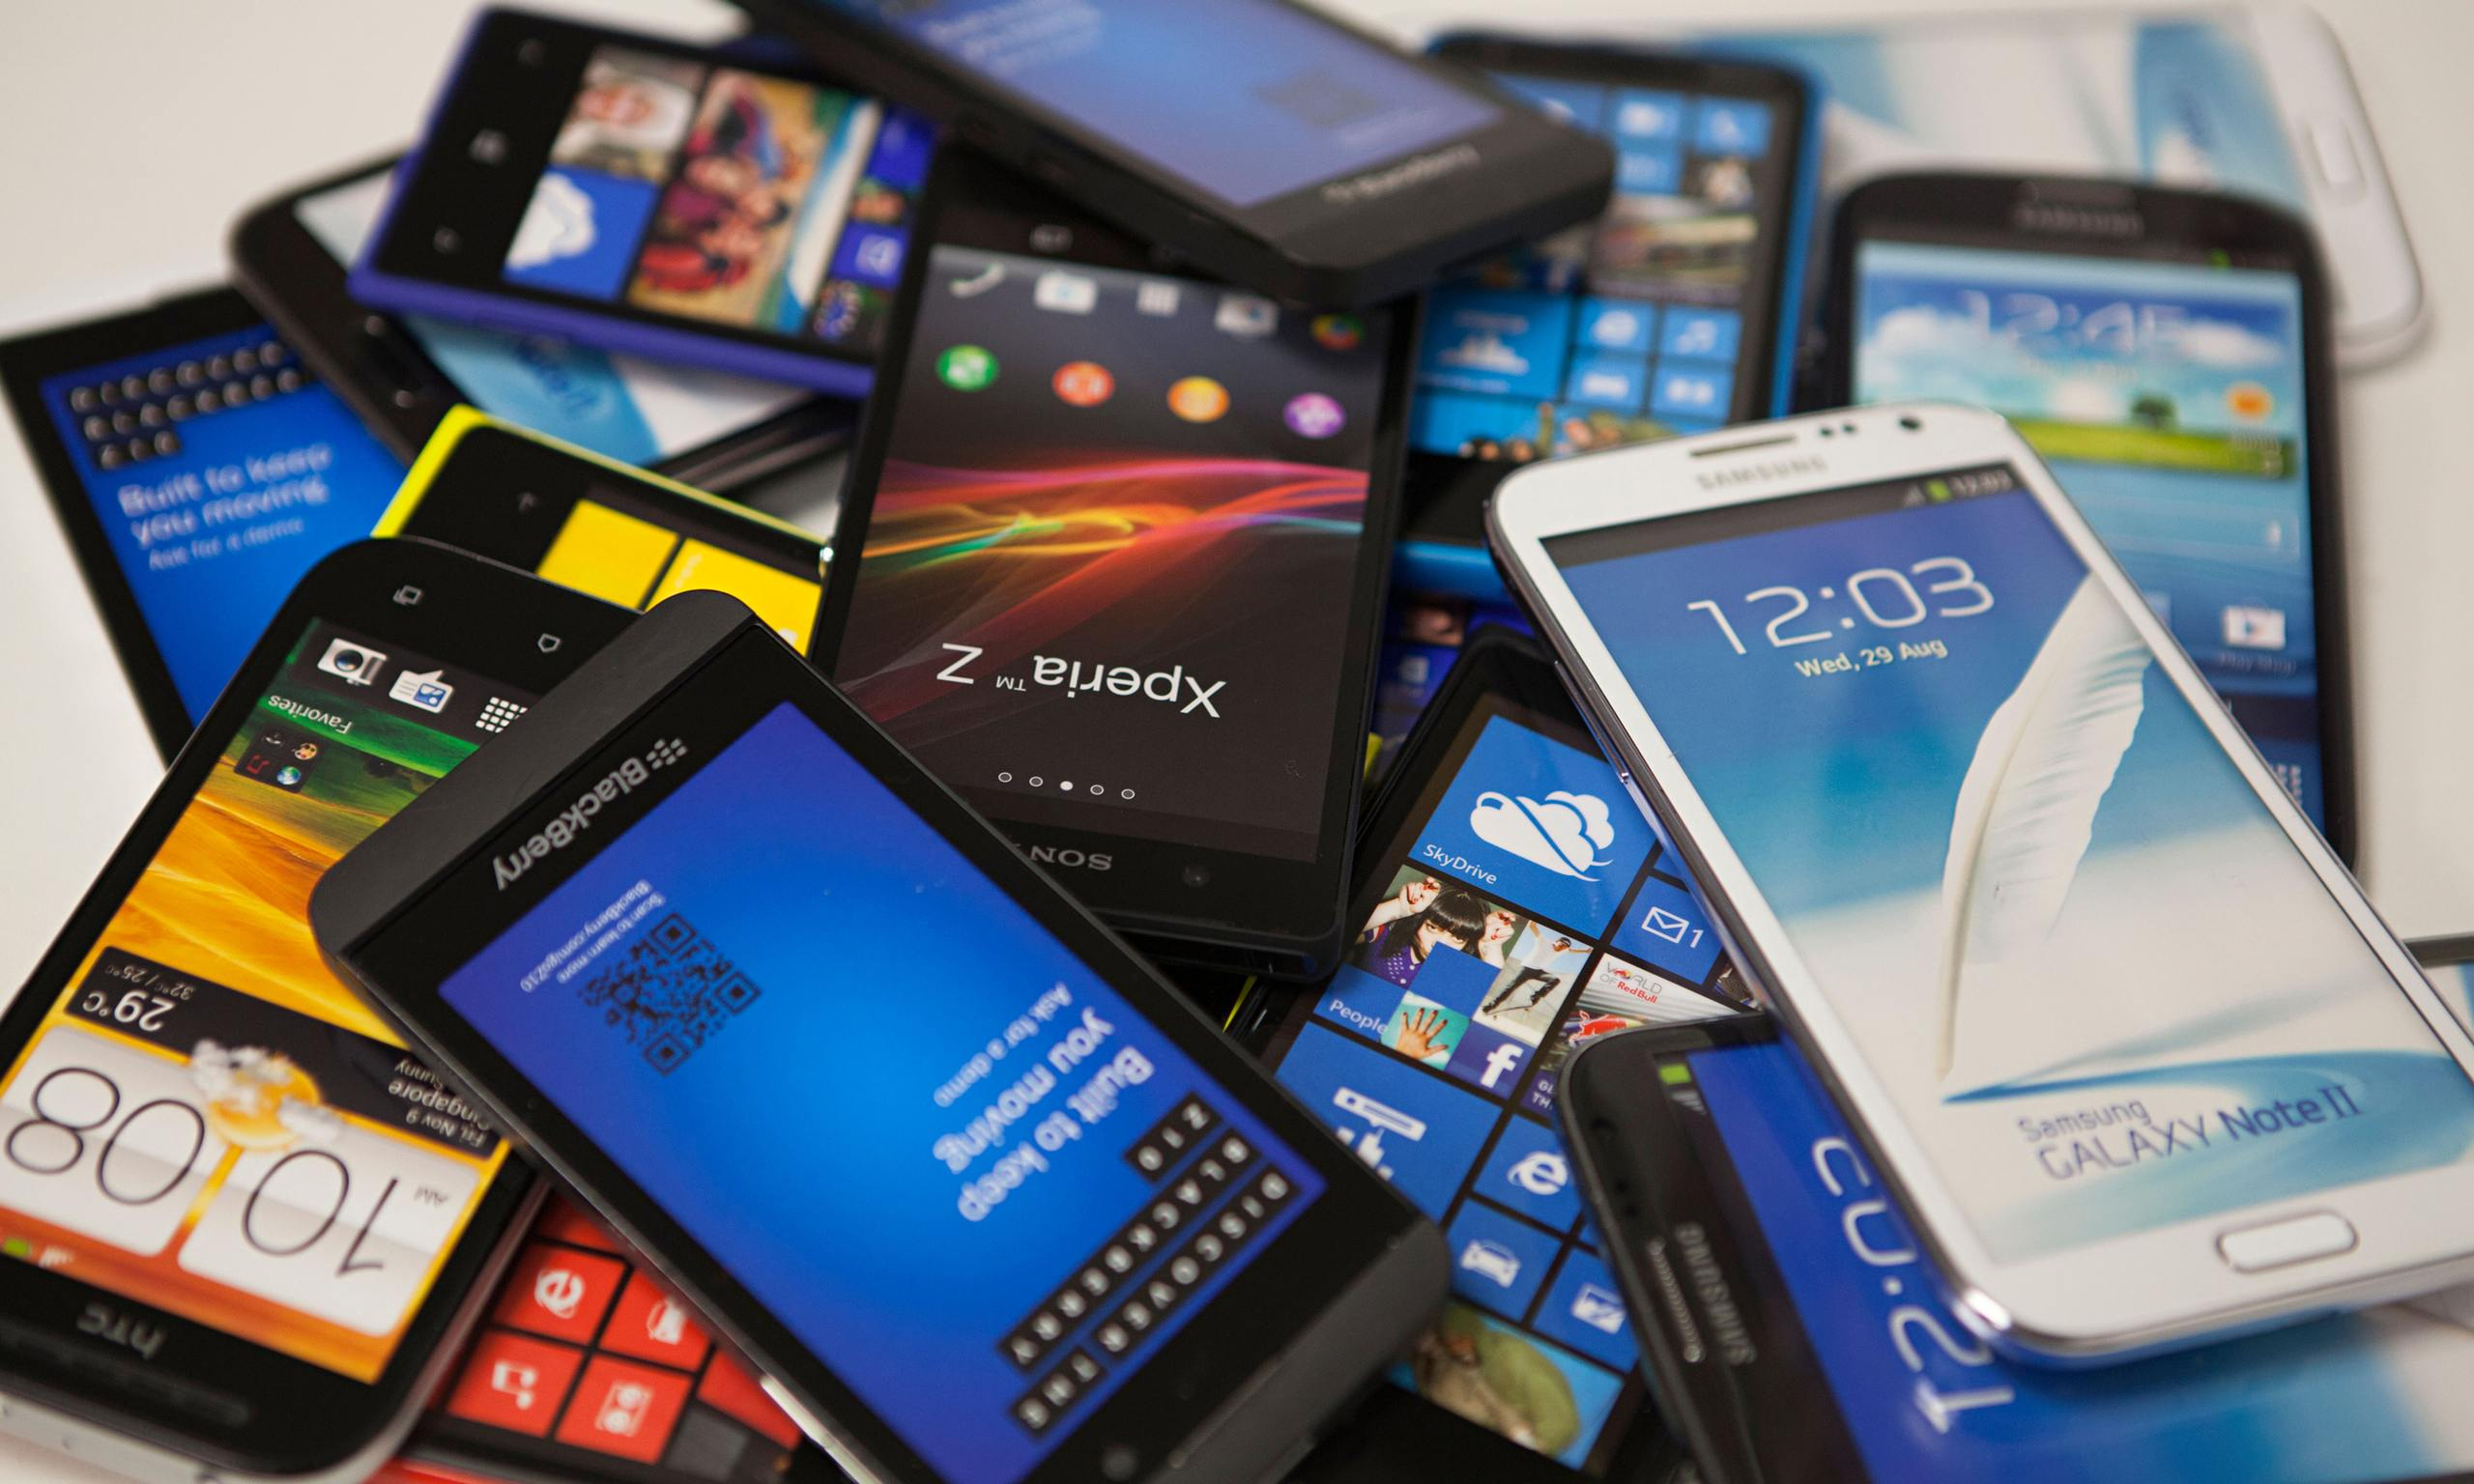
\includegraphics[scale=0.056]{./figures/cellphones.jpg}}
    \end{center}
  }
  
  \begin{columns}[T]
    \begin{column}{.3\textwidth}
      \uncover<2-4>{
        \begin{center}
	    \advance\leftskip-0.2cm
	      {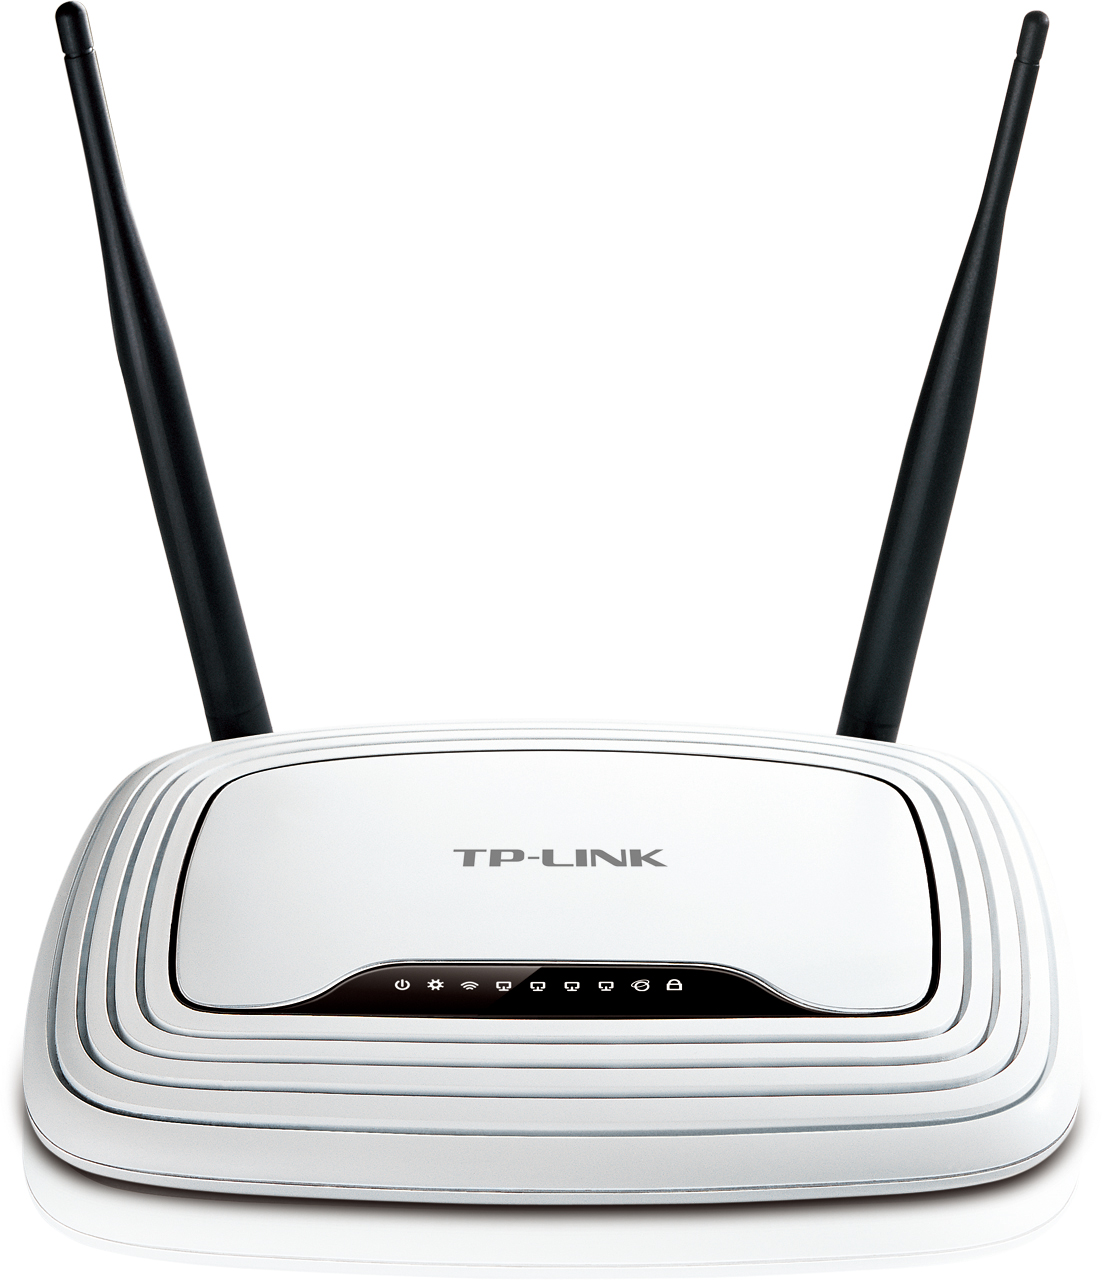
\includegraphics[scale=0.052]{./figures/tplink.jpg}}
        \end{center}
      }
    \end{column}
    
    \begin{column}{.18\textwidth}
      \uncover<3-4>{
        \begin{center}
	      \advance\leftskip-0.2cm
	      {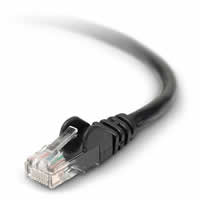
\includegraphics[scale=0.31]{./figures/cable-red.jpg}}
        \end{center}
      }
    \end{column}
    
    \begin{column}{.3\textwidth}
      \uncover<4-4>{
        \begin{center}
	      \advance\leftskip-0.2cm
	      {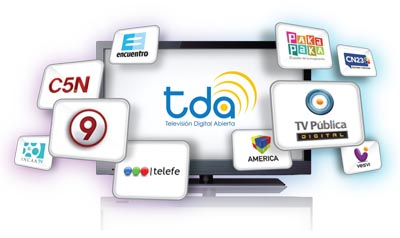
\includegraphics[scale=0.31]{./figures/tda1.png}}
        \end{center}
      }
    \end{column}
  \end{columns}
\end{frame}

\begin{frame}{¿Como funciona?}
  \begin{columns}[T]
    \begin{column}{.3\textwidth}
      \begin{itemize}
        \item<2-> Divide la información en múltiples frecuencias
        \item<3-> Bandas de frecuencia solapadas
      \end{itemize}
    \end{column}
    
    \begin{column}{.7\textwidth}
      \uncover<2->{
        \alt<2>{
          \begin{center}
            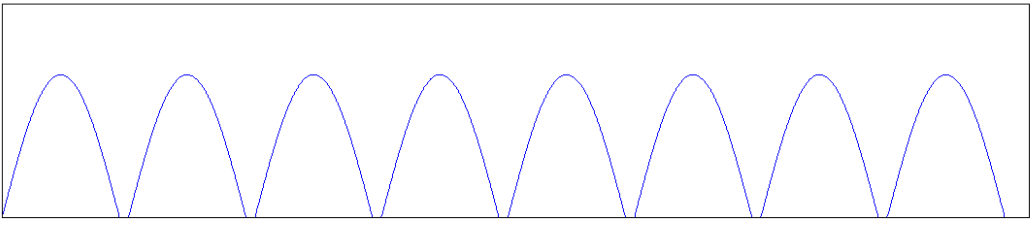
\includegraphics[scale=0.17]{./figures/freq_mux.png}
          \end{center}
        }{
        %\uncover<4->{
          \begin{center}
            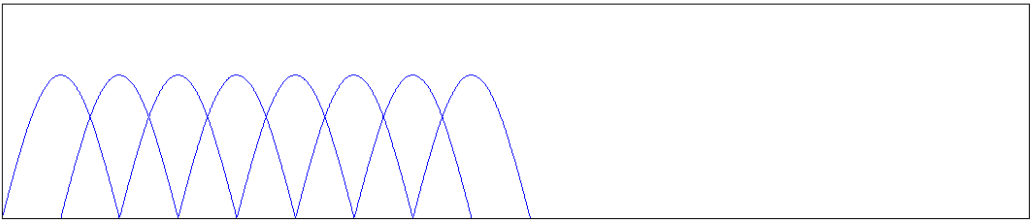
\includegraphics[scale=0.17]{./figures/freq_ort.png}
          \end{center}
        }
      }
    \end{column}
  \end{columns}
  
  \begin{itemize}
    \item<4-> Necesito sintonizar todas las frecuencias
    \begin{itemize}
      \item<5-> Se puede implementar en hardware
      \item<7-> Se puede implementar en software
    \end{itemize}
  \end{itemize}
  
  \begin{columns}[T]
    \begin{column}{.5\textwidth}
      \uncover<6->{
        \begin{center}
          \advance\leftskip-0.2cm
          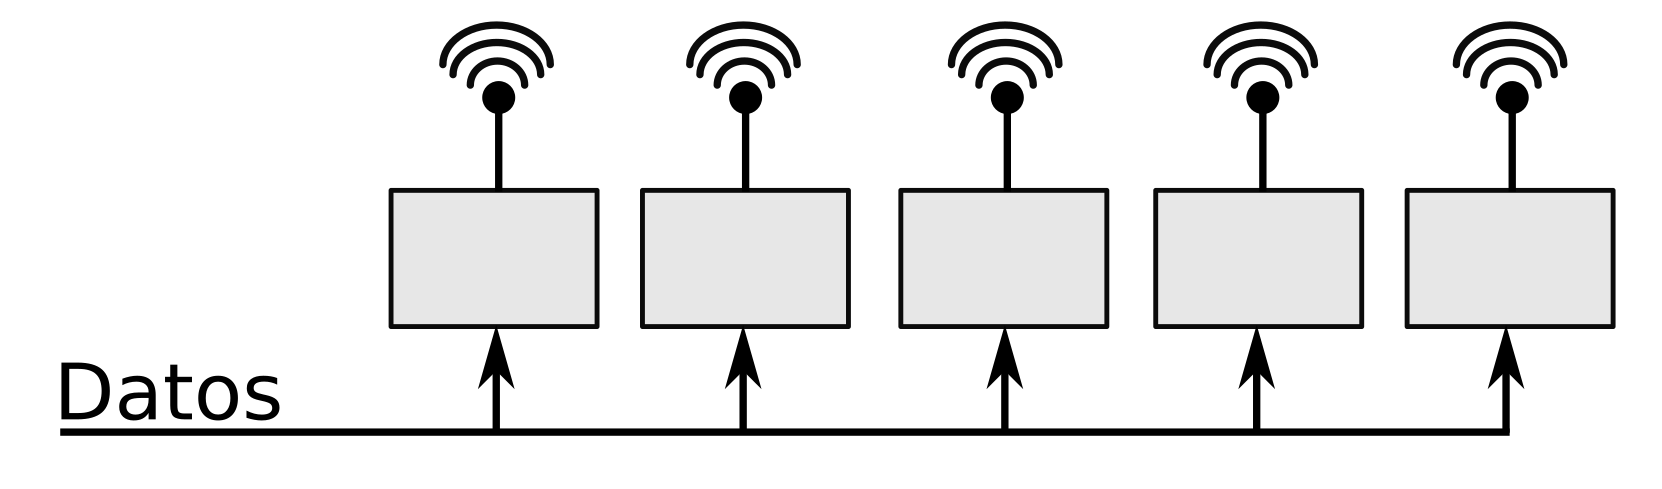
\includegraphics[scale=0.26]{./figures/hard_mod.png}
        \end{center}
      }
    \end{column}
    
    \begin{column}{.5\textwidth}
      \uncover<8->{
        \begin{center}
          \advance\leftskip-0.2cm
          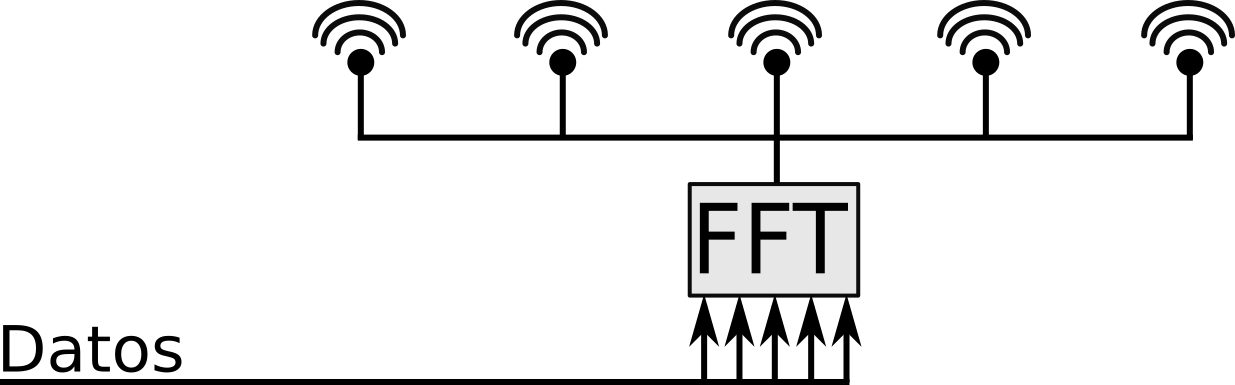
\includegraphics[scale=0.26]{./figures/soft_mod.png}
        \end{center}
      }
    \end{column}
  \end{columns}
  
  
\end{frame}

\begin{frame}{FFT}
  \Fontit
  \begin{itemize}
    \item<1-> Transformada rápida de Fourier
    \item<2-> Sumas/restas y multiplicaciones
    \item<3-> Cada salida = suma y resta de todas las entradas 
  \end{itemize}
  
  \vfill
  
  \uncover<3->{
    \begin{center}
      \advance\leftskip-0.2cm
      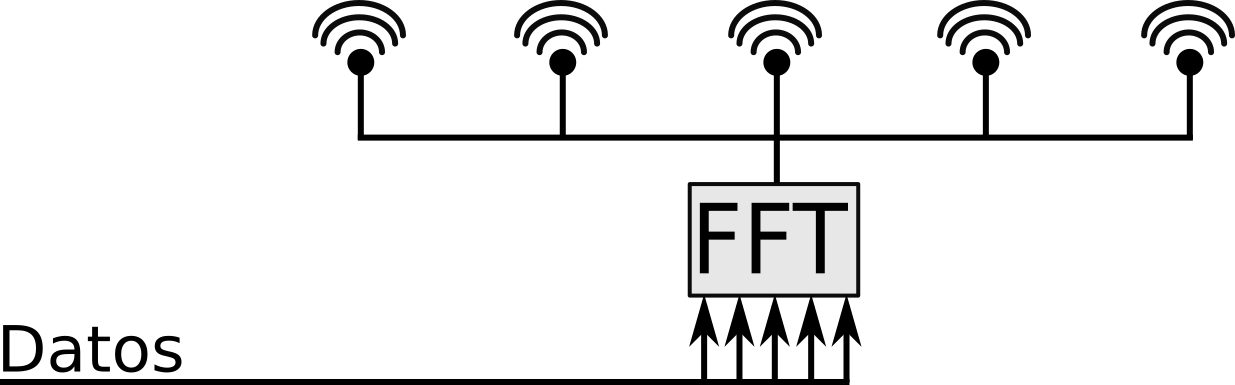
\includegraphics[scale=0.30]{./figures/soft_mod.png}
    \end{center}
  }
      
\end{frame}

\begin{frame}{FPGA}

\begin{columns}[T]
  \begin{column}{.2\textwidth}
      \uncover<2->{
        \alt<2>{
        \begin{center}
          \advance\leftskip-0.2cm
          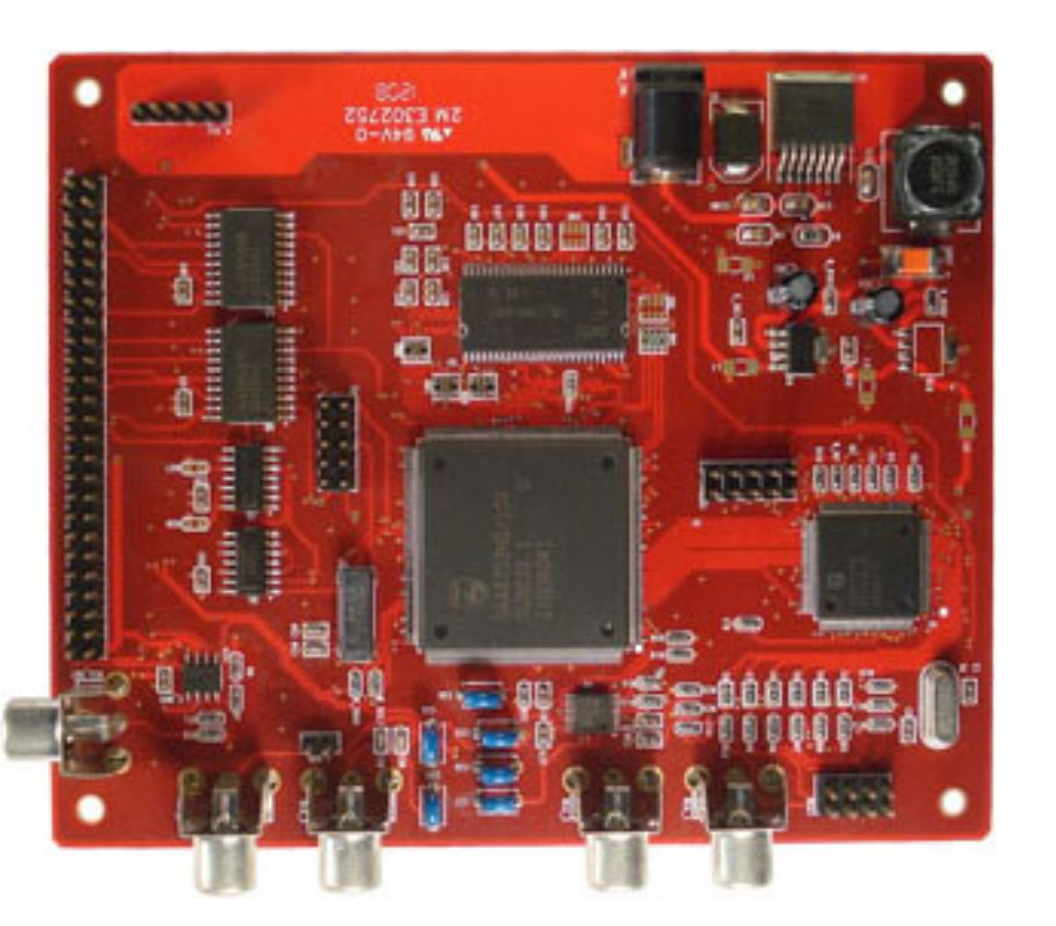
\includegraphics[scale=0.20]{./figures/circ_good.png}
        \end{center}
        }{
        \begin{center}
          \advance\leftskip-0.2cm
          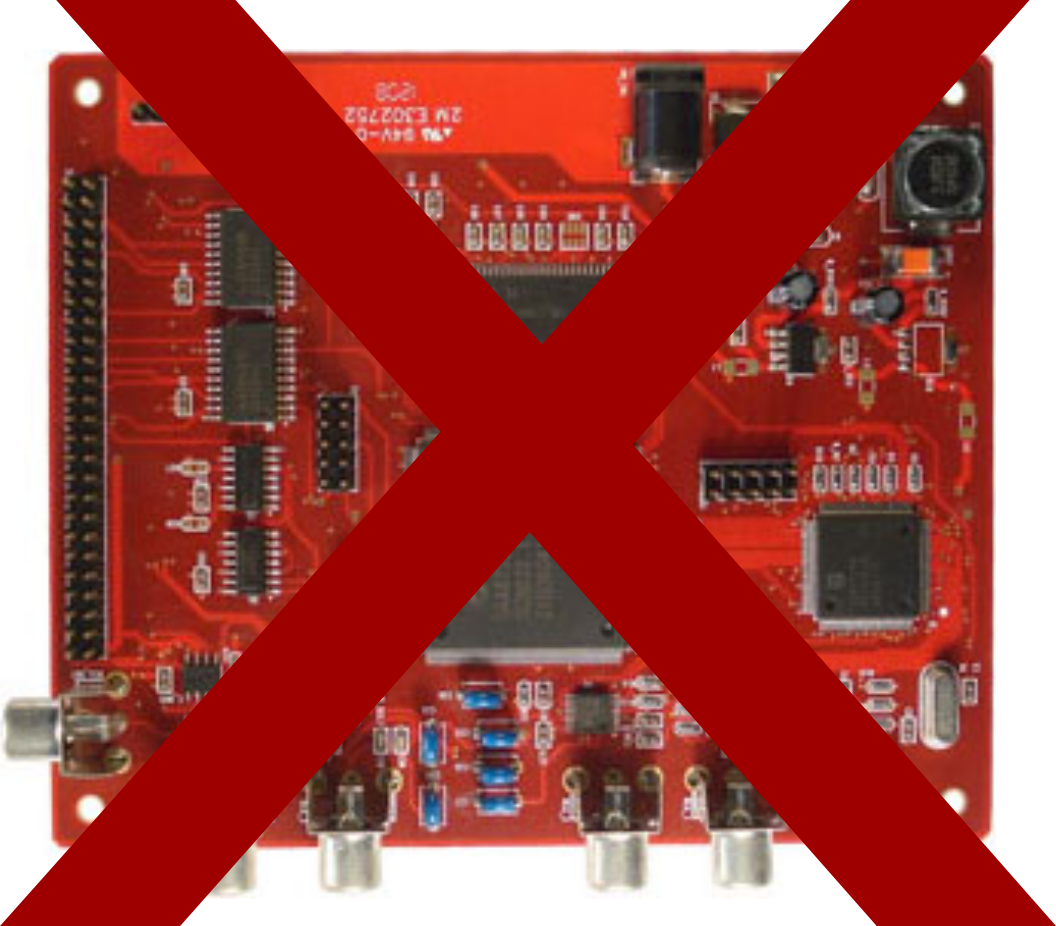
\includegraphics[scale=0.20]{./figures/circ_bad.png}
        \end{center}
        }
      }
    \end{column}
    \begin{column}{.2\textwidth}
      \uncover<4->{
        \begin{center}
          \advance\leftskip-0.2cm
          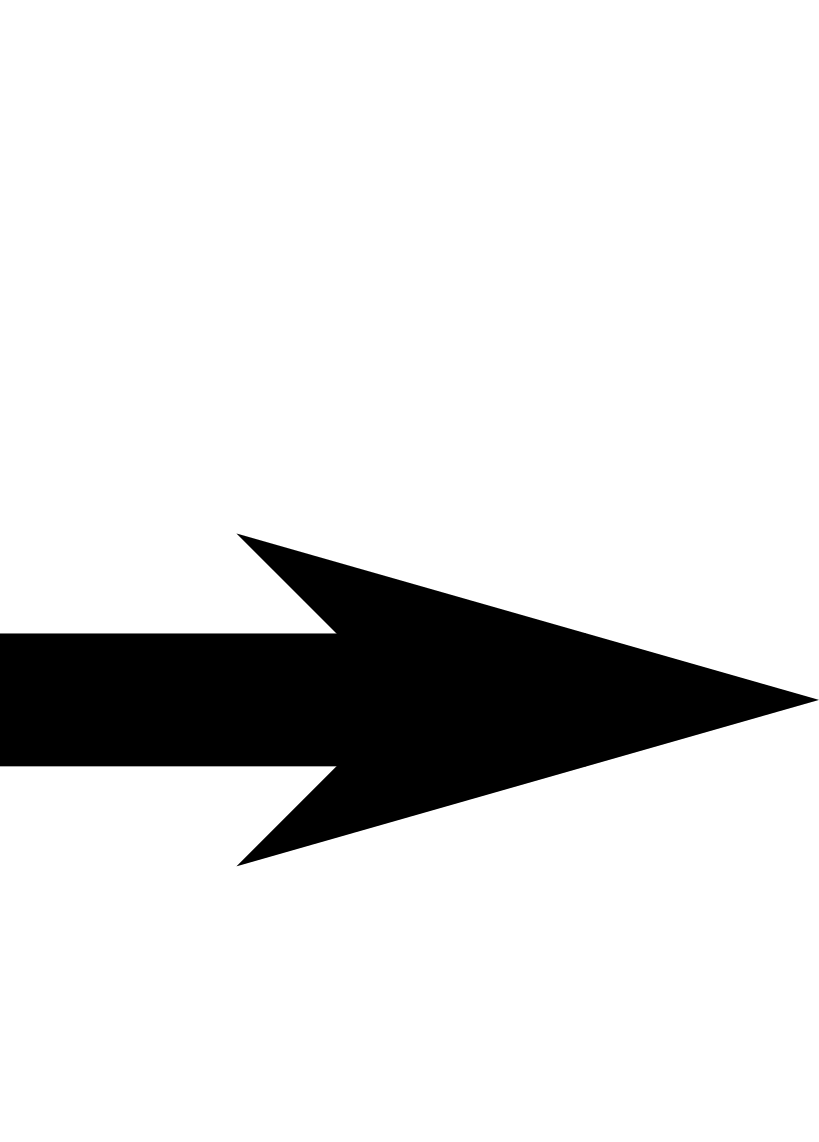
\includegraphics[scale=0.13]{./figures/flecha.png}
        \end{center}
       }
    \end{column}
    
    \begin{column}{.2\textwidth}
      \uncover<5->{
        \alt<5>{
        \begin{center}
          \advance\leftskip-0.2cm
          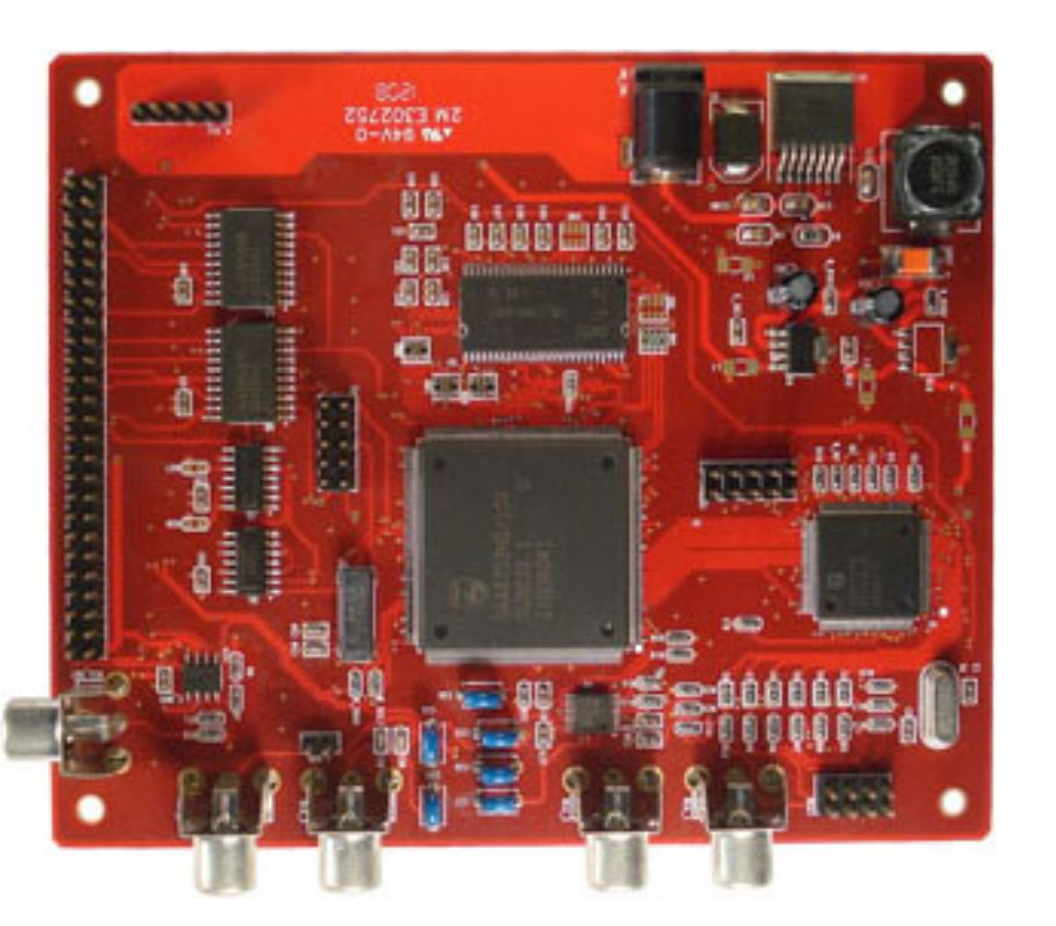
\includegraphics[scale=0.20]{./figures/circ_good.png}
        \end{center}
        }{
        \begin{center}
          \advance\leftskip-0.2cm
          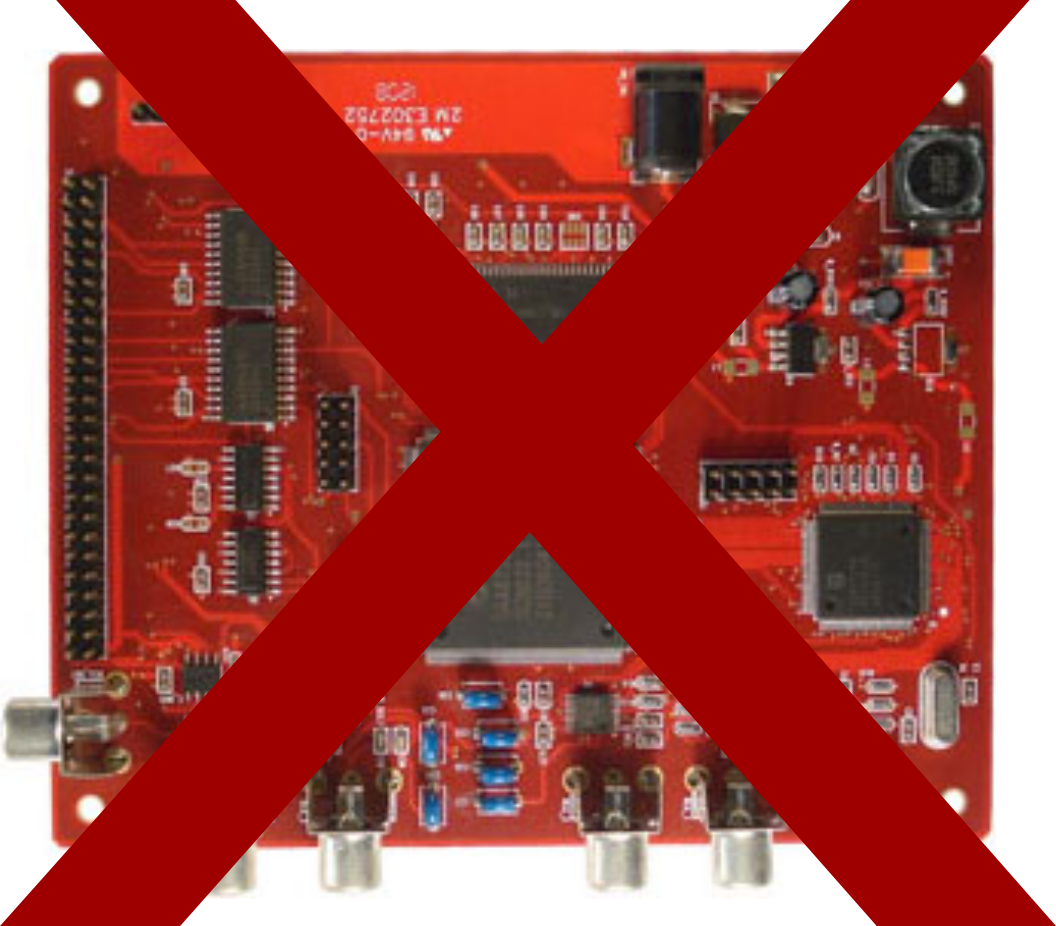
\includegraphics[scale=0.20]{./figures/circ_bad.png}
        \end{center}
        }
      }
    \end{column}
    \begin{column}{.2\textwidth}
      \uncover<6->{
        \begin{center}
          \advance\leftskip-0.2cm
          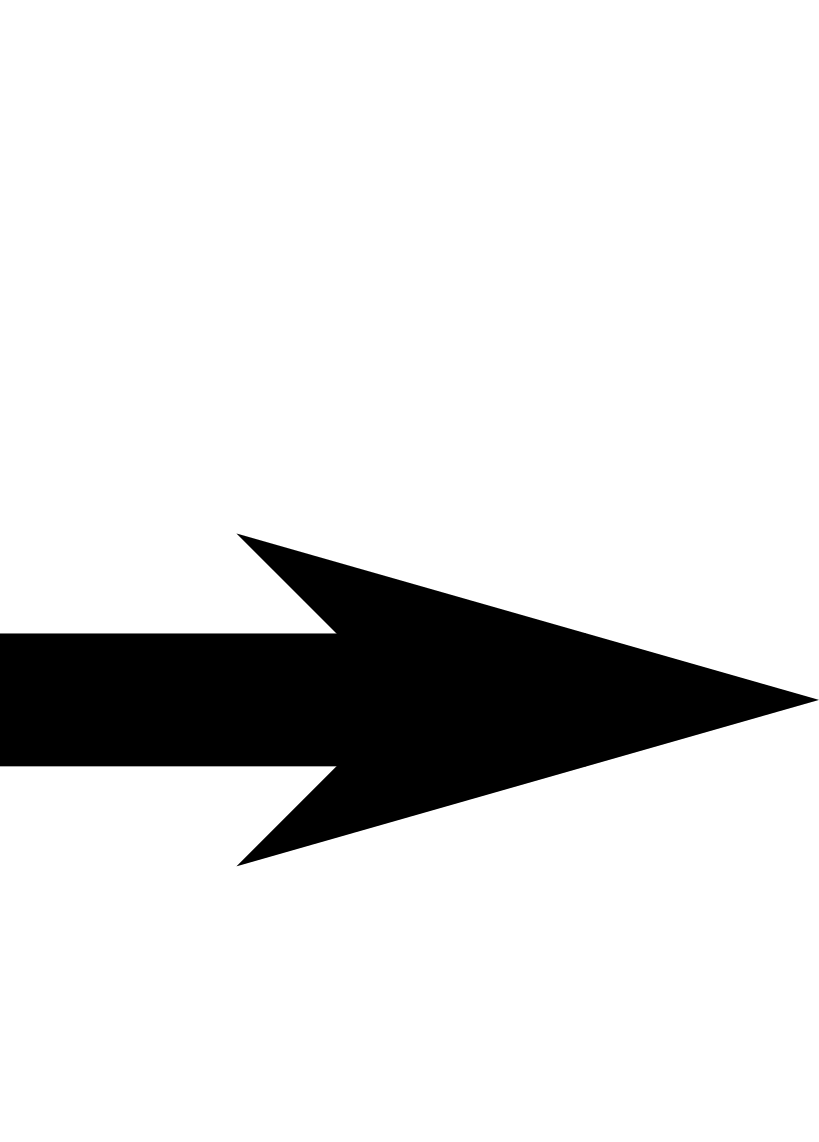
\includegraphics[scale=0.13]{./figures/flecha.png}
        \end{center}
       }
    \end{column}
    
    \begin{column}{.2\textwidth}
      \uncover<7->{
%         \alt<7>{
        \begin{center}
          \advance\leftskip-0.2cm
          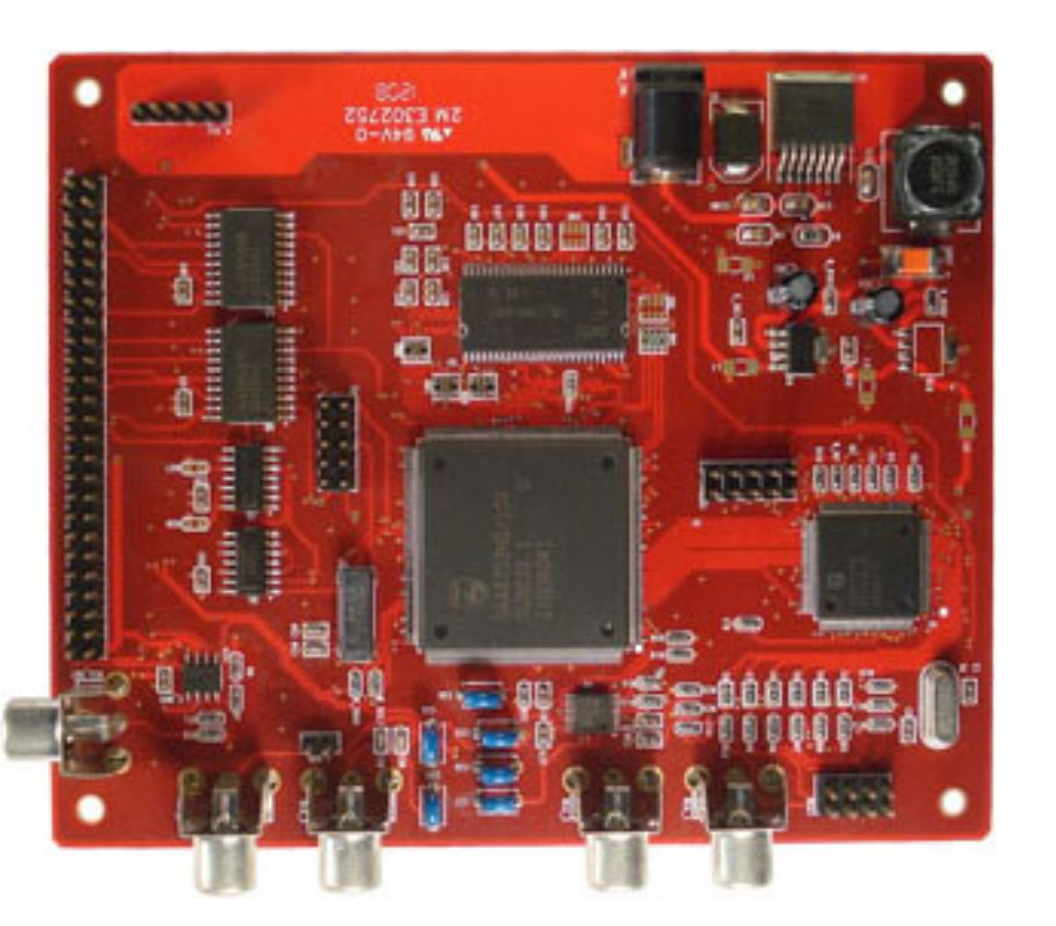
\includegraphics[scale=0.20]{./figures/circ_good.png}
        \end{center}
%         }{
%         \begin{center}
%           \advance\leftskip-0.2cm
%           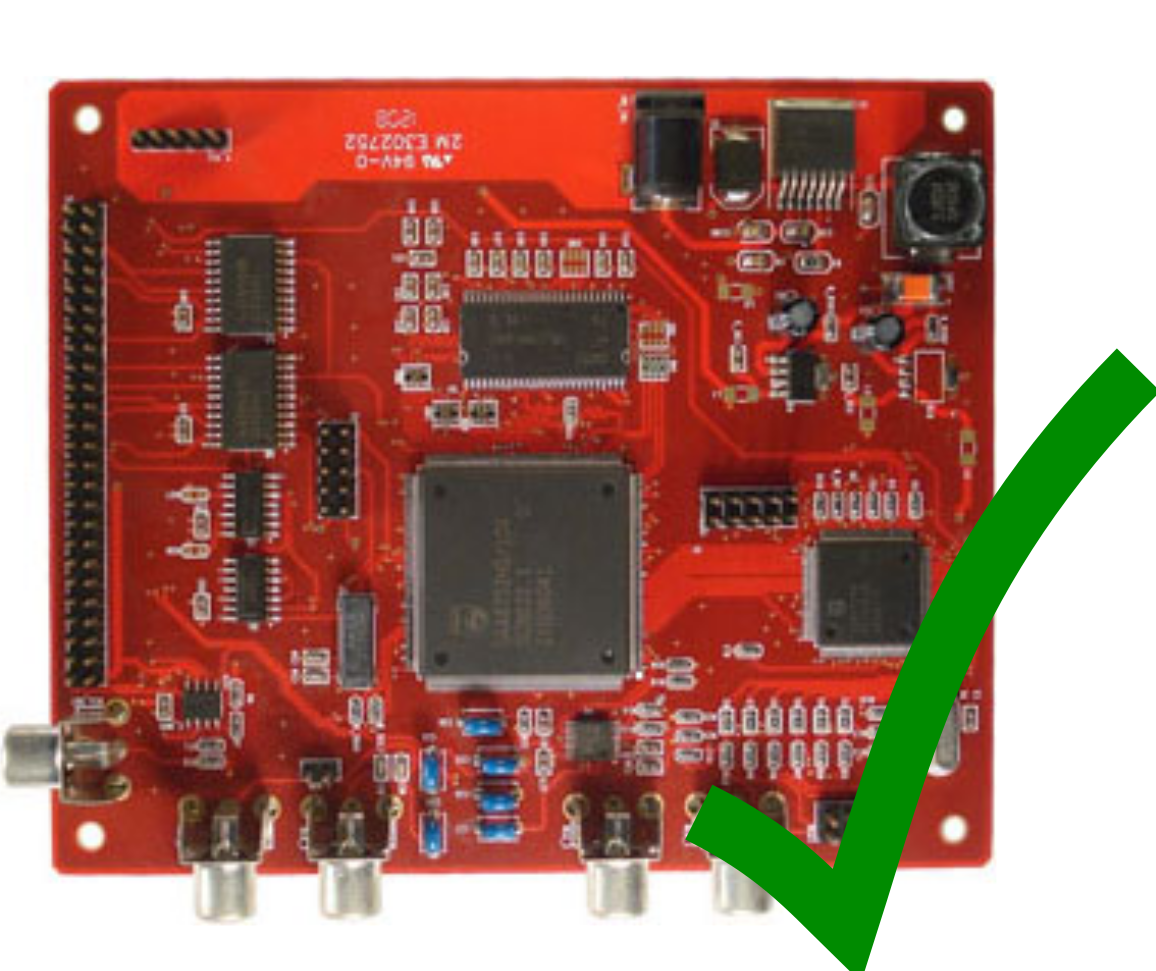
\includegraphics[scale=0.20]{./figures/circ_tick.png}
%         \end{center}
%         }
      }
    \end{column}
    
    
    
  \end{columns}
  
  \vfill
  
  \uncover<8->{
	  \begin{center}
		  \advance\leftskip-0.2cm
		  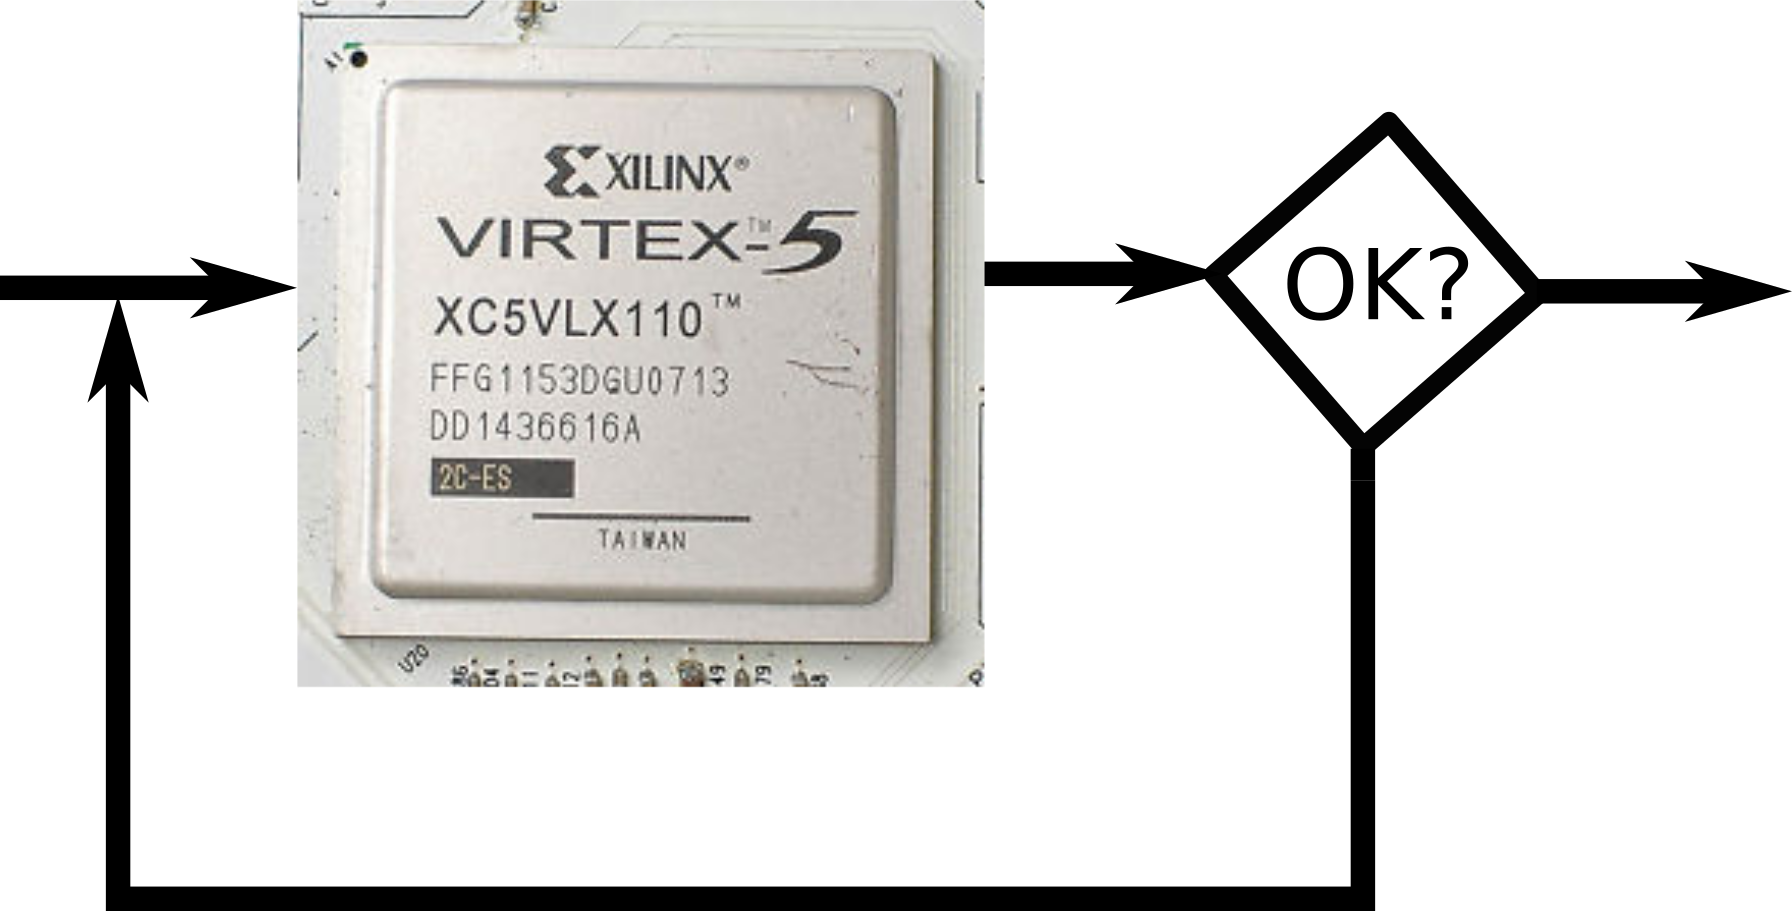
\includegraphics[scale=0.26]{./figures/fpga_design.png}
	  \end{center}
  }

\end{frame}

\begin{frame}
	\begin{center}
	\Huge MOTIVACIÓN Y OBJETIVOS
	\end{center}
\end{frame}

\subsection{Motivacion}

\begin{frame}{Motivación}
  \Fontit
  \begin{itemize}
    \item<1-> El avance de los sistemas de radio definidos por software
    \item<2-> La flexibilidad que brindan las FPGAs para implementar sistemas complejos
    \item<3-> La necesidad de sistemas de comunicaciones de código libre, eficientes y económicos
    \item<4-> Aportar al desarrollo de un sistema de telecomunicaciones dentro del LSE
    de la facultad
  \end{itemize}
\end{frame}

\subsection{Objetivos}
\begin{frame}{Objetivos}
  \Fontit
  \begin{itemize}
    \item<1-> Diseñar un modulador/demodulador para un sistema de telecomunicaciones definido por
    software.
    \only<2-5>{\begin{itemize}
      \Fontitit
      \item<2-5> Desempeño
      \item<3-5> Escalabilidad
      \item<4-5> Versatilidad
      \item<5-5> Tamaño reducido
    \end{itemize}} 
    \item<6-> Realizar una evaluación de desempeño
    \only<7-10>{\begin{itemize}
      \Fontitit
      \item<7-10> Funcionamiento
      \item<8-10> Ruido / error
      \item<9-10> Distorsión armónica
      \item<10-10> Recursos
    \end{itemize}} 
    \item<11-> Realizar una comparativa con desarrollos de terceros para evaluar el diseño realizado
    \item<12-> Proponer trabajos futuros para continuar y mejorar el diseño.
 \end{itemize}    
\end{frame}
